\section{Proposed Method}
\label{sec:method}

A complete pipeline of Deep Shape-Aware Network (DSAN) is illustrated in Figure~\ref{FigDSAN}.
The framework is trained end-to-end and consists of three key components:
1) a deep multi-task network based on FCN,
2) proposed split max pooling and
3) piecewise fusion strategy to generate the final segmentation mask.
%

Given an input image, the first part is a multi-task FCN to simultaneously predict an objectness score and shape parameters at each pixel (Sec.~\ref{sec:multi-task-fcn}).
Then the outputs of multi-task FCN are optimized with each other by a split max pooling layer (Sec.~\ref{sec:split-max-pooling}) and further integrated into final segmentation task using a piecewise fusion step (Sec.~\ref{sec:fusion}).

\begin{figure*}
    \begin{center}
        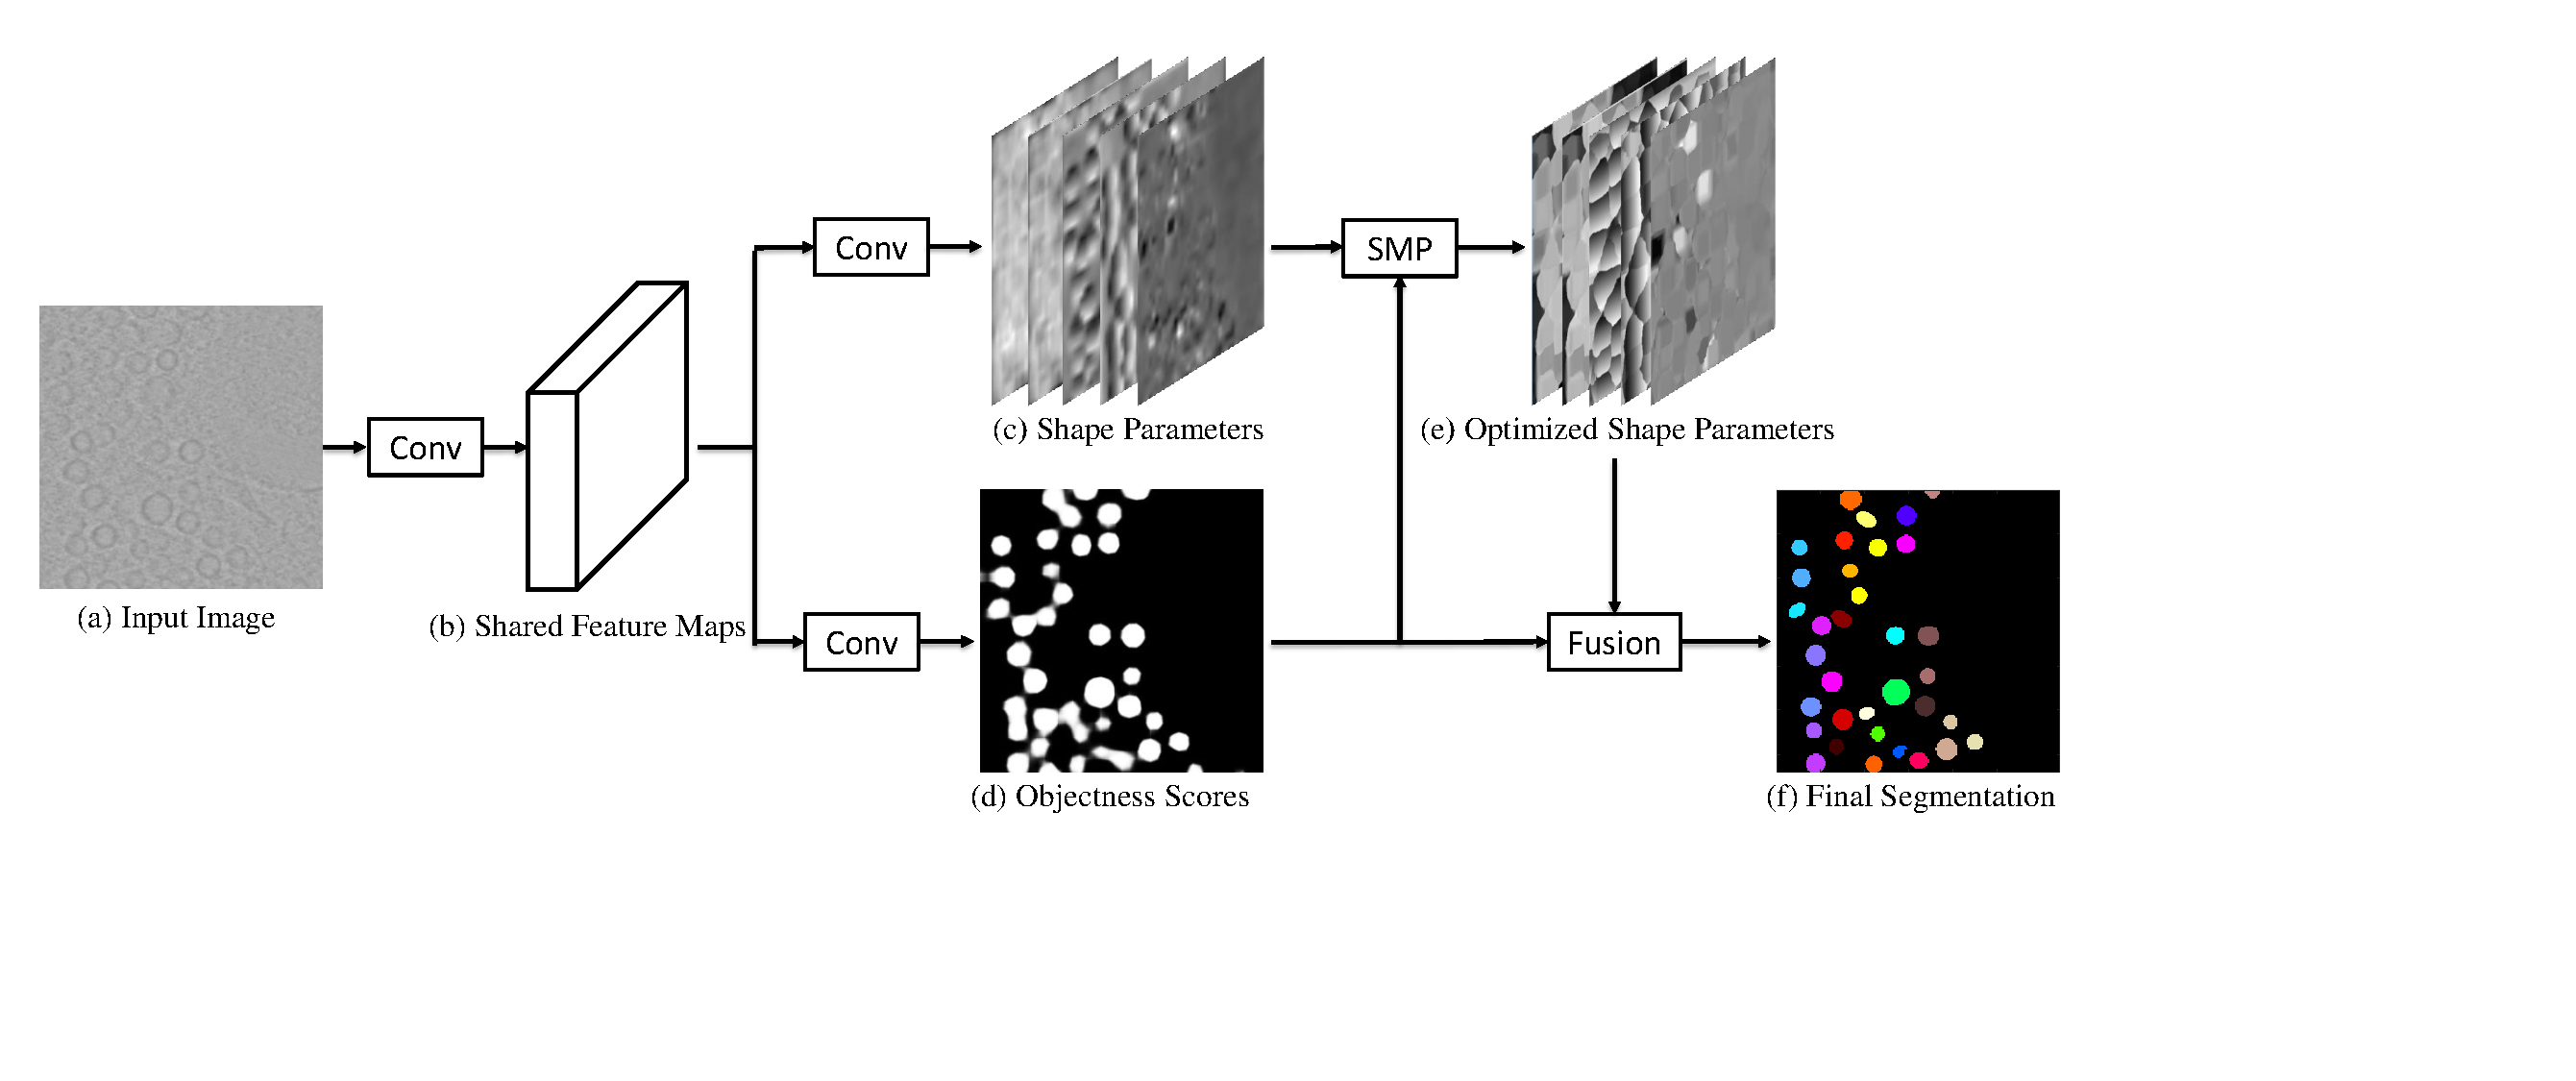
\includegraphics[width=6.7in]{figures/FigDSAN.pdf}
    \end{center}
    \caption{Overview of our proposed DSAN. Given an image (a), a multi-task network simultaneously predicts objectness scores (d) and shape parameters of objects (d) by successive convolutions denoted by Conv.
    For convenience, operations, such as pooling and ReLu, have been omitted.
    Then a split max pooling (SMP) is applied to pool (c) with (d) and output new shape parameters (e).
    Finally, segmentation mask (f) is obtained by fusing (Fusion) objectness scores (d) and shape parameters (e).}
    \label{FigDSAN}
\end{figure*}
\subsection{Multi-task FCN}
\label{sec:multi-task-fcn}

The architecture of our multi-task learning network is shown in Figure~\ref{FigDSAN}.
It simultaneously predicts an objectness map $P$ and several auxiliary maps $\{T_k\}_{k=1,\ldots,K}$ as complementary information.
The feature extracting part is shared and can be replaced by any networks, such as DeepLab~\cite{Chen2014a}, ResNet~\cite{Zhao2016} or recent DenseNet~\cite{Huang2016}. 
As FCN is still commonly used and suffers from more serious touching problem in biomedical segmentation \cite{Chen2015,Lieman-Sifry2017,Xu2016,Chen2016b}, we select the DeepLab model for feature extracting in order to demonstrate our superiority on resolving touching and coarse boundary problem.

Then, the feature maps extracted by last shared convolution layer are fed into two individual branches.
In each branch, successive two convolution layers are applied to the input feature maps with stride $1$ and respective kernel size $3\times 3$and $1\times 1$.
Then the outputs of each branch are upsampled to match the original image using bilinear interpolation.
During training, the parameters of shared layers are jointly optimized, while the parameters of two branches are updated independently.

Instead of directly predicting contour probabilities in \cite{Chen2016a,Xu2016}, we choose the parameterized expression of objects shape as complementary information, which emphasizes more on the overall shape of objects to be segmented.
For example in our task for vesicle segmentation, the ellipse shape is selected as our prior shape knowledge and formulated by parameters $\{\theta, \mu_c, \nu_c, a, b\}$.
$\theta$ is the rotated angle of major axis from $x-$axis.
$(\mu_c, \nu_c)$ are the coordinates of ellipse center.
And $a$, $b$ are respectively the lengths of major and minor axis.
With these definitions, $K$ is set to be $5$ and each $T_k$ predicted one of the five parameters.
Therefore, predicted $T_k$ at pixel $i$ make up a parameters vector $\mathbf{t}_i\in R^5$, formulating the shape of a nearest object of $i$.
For better regression, the shape parameters are further normalized by image width $W$ and height $H$ so that they fall in $[0,1]$:
\begin{eqnarray}\label{EqPara}
\begin{aligned}
\mathbf{t}_{i} = \{\theta,\frac{\mu-\mu_c}{W},\frac{\nu-\nu_c}{H},\frac{a}{H},\frac{b}{H}\}
\end{aligned}
\end{eqnarray}
where $(\mu, \nu)$ are spatial coordinates of pixel $i$.

For an input image, The objective function of our multi-task FCN is defined by:
\begin{eqnarray}\label{EqLoss}
\begin{aligned}
L(P,\{T_k\}) =& \frac{1}{N}(\sum_{i}L_{cls}(P_i,P^*_{i})+\\
&\lambda\sum_{i}\sum_{k}P^*_{i}L_{reg}(T_{k,i},T^*_{k,i}))\\
\end{aligned}
\end{eqnarray}
where $N$ is the total number of pixels.
$P^*_i$ and $T^*_{k,i}$ are the ground truth of objectness score and $k$-th shape parameter at pixel i.
The classification loss $L_{cls}$ is the soft-max loss and regression loss $L_{reg}$ is defined by
\begin{eqnarray}
\label{EqSmoothL1}
\begin{aligned}
L_{reg}(t_1,t_2) =\left\{\begin{array}{cc}
0.5(t_1-t_2)^2&if~|t_1-t_2|<1\\
|t_1-t_2|-0.5&else\\
\end{array}\right.
\end{aligned}
\end{eqnarray}
which is the smoothed $L_1$ loss for robust regression in \cite{Ren2015}.

Especially in Eq.~\ref{EqLoss}, we only consider the regression loss with positive $P^*_i$, because most $T_{k,i}$ with negative $P^*_i$ will be abandoned in next section by proposed split max pooling.
And $\lambda$ is a balancing weight between $L_{cls}$ and $L_{reg}$.

\subsection{Split Max Pooling}
\label{sec:split-max-pooling}

Obtained from two individual branches of multi-task FCN, the predicted shape parameters in auxiliary maps are not accurate enough to optimize the objects shape predicted in objectness map.
This is caused by different perception field needed by different position to explore the complete shape of a nearest object.
Usually in an auxiliary map, predictions in central region of an object are more accurate than those in boundary region, which needs a lager perception filed to learn the whole object shape.
To this end, we introduce a novel split max pooling (SMP) to improve the accuracy of auxiliary predictions in boundary region of objects by utilizing the complementary information in objectness scores.
Different from conventional max pooling, our SMP takes two maps as inputs and pools one with the other one.
And its back propagation can further benefits both inputs by exploring the inherent association between them.

A conventional pooling operation can be expressed as
\begin{eqnarray}\label{pooling}
\begin{aligned}
y_{j} = \sum_{i\in \mathcal{N}_{j}} \omega_{i}x_{i}
\end{aligned}
\end{eqnarray}
where $\mathcal{N}_{j}$ is a neighbor region of pixel $j$ according to the sliding window, and $\omega_{i}$ is the weight of pixel $i$.
For traditional max pooling, $\omega_i \in \{0,1\}$ is a binary indicator for that if $x_i$ is the maximum in the local region.
There is only one pixel in the neighborhood has $\omega=1$ and all the others have $\omega=0$.
For an average pooling, all pixels in the local window take the identical weight $\omega=\frac{1}{N}$, where $N$ is the total number of pixels in the local region $\mathcal{N}$.
Intuitively, $\omega$ acts like an $``$indictor" determining which $x$ should be propagated to next layer.

\begin{figure}
    \begin{center}
        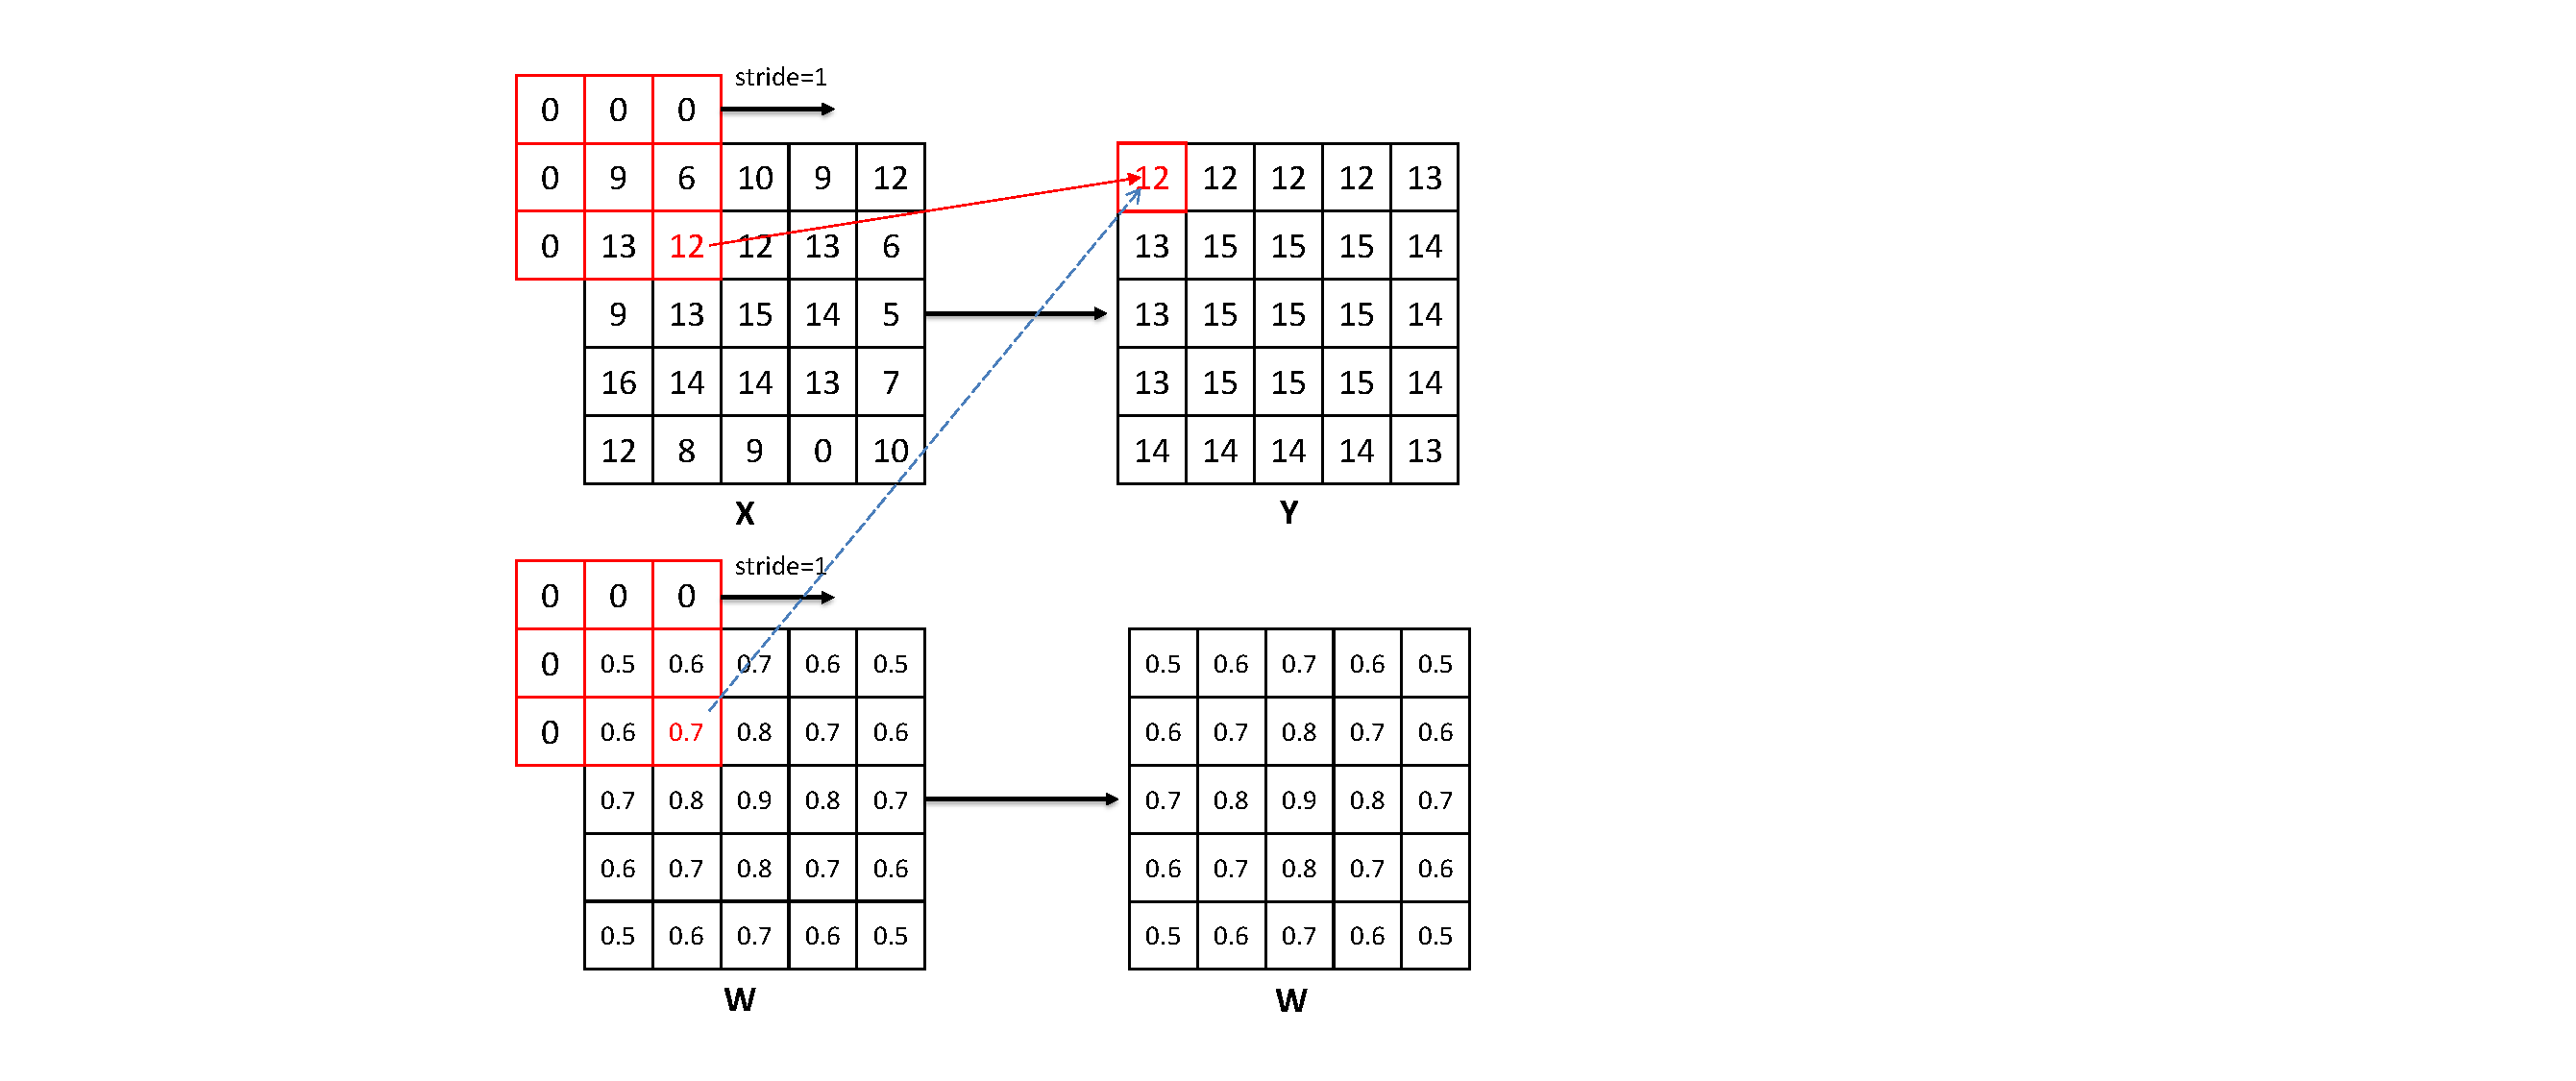
\includegraphics[width=3.4in]{figures/FigSMP.pdf}
   %\includegraphics[width=0.8\linewidth]{egfigure.eps}
    \end{center}
    \caption{An example of joint max pooling.
        Two windows of same size synchronously slide on $\mathbf{X}$ and $\mathbf{W}$.
       The elements in top window will be propagated the element under the indicator of bottom window.}
    \label{FigSMP}
\end{figure}

Based on this observation, we proposed a split max pooling (SMP) operation, of which the $\omega$ is generated from an independent input, rather than $x$.
Explicitly, our SMP takes two inputs: $X$ and $W$, respectively corresponding to the auxiliary map $T_k$ and objectness map $P$ in our task.
During forward propagation, two windows with same size, denoted by $\mathcal{N}^{x}$ and $\mathcal{N}^{\omega}$, synchronously slide on $X$ and $W$.
%$\mathcal{N}^{x}$ and $\mathcal{N}^{\omega}$ has the same perception field $\mathcal{N}$ on different input maps.
The $\mathcal{N}^{x}$ is the pooling window, while $\mathcal{N}^{\omega}$ is the decision window.
The pooling strategy in $\mathcal{N}^{x}$ will be determined according to the elements in $\mathcal{N}^{\omega}$.
For example, the forward propagation of split max pooling can be expressed by:
\begin{eqnarray}\label{smp}
\begin{aligned}
y_{j} &= \sum_{i\in \mathcal{N}_{j}}x_{i}\hbar(\omega_{i},\mathcal{N}^{\omega}_{j})\\
\hbar(\omega_{i},\mathcal{N}^{\omega}_{j})&=\left\{\begin{array}{cc}
1&if~\omega_{i}\geq max(\mathcal{N}^{\omega}_{j})\\
0&else\\
\end{array}\right.
\end{aligned}
\end{eqnarray}
Here, $\hbar(\cdot)$ is a threshold function to transform $\omega_i$ to be binary.
$max(\cdot)$ returns the maximum value of the input set.

A simple example is illustrated in Figure~\ref{FigSMP}.
After split max pooling, only $x_i$ with larger $\omega_i$ can be propagated to next layer and fill the whole $\mathbf{Y}$ in Figure~\ref{FigSMP}.
When the SMP is iterated several times, all the elements in $Y$ will be substituted by the $x_i$ with maximum $\omega_i$.

For our segmentation task, it is reasonable to believe that objectness score $p_i$ obtained in central region of an object are probably the local maximum.
Therefore, SMP is able to replace the predicted shape parameters $T_{k,i}$ in boundary region with the neighbouring $T_{k,j}$ of central area.
And the pooling size and iteration times of SMP change the influence range of a $T_{k,i}$ with maximum $P_i$.
In our experiments, the pooling stride is fixed to be $1$ to maintain an unchanged resolution of output map.

Another contribution of our SMP is that the residual error can be correctly back propagated to its inputs.
This makes it a trainable layer in any network architecture and our SCNN become a fully trainable system.
Defining $L$ as the residual error, the back propagation for $x_{i}$ can be expressed by:
\begin{eqnarray}\label{bpx}
\begin{aligned}
\frac{\partial L}{\partial x_{i}}=\frac{1}{m}\sum\limits_{j\in\mathcal{N}_{i}}\frac{\partial L}{\partial y_{j}}\hbar(\omega_{i},{\mathcal{N}}^{\omega}_{j})\\
\end{aligned}
\end{eqnarray}
where $\mathcal{N}^{\omega}_{j}$ is the neighbor region centered at position $j$ of $W$ and $m$ is the number of elements in $\mathcal{N}_{i}$.
Similar to forward propagation of original max pooling, Eq.~\ref{bpx} converge the gradients $\frac{\partial L}{\partial y_{j}}$ into the $x_{i}$ that has a local maximum $\omega_{i}$.
As most residual error of $T_{k,i}$ have been converged at the pixels with maximum $P_i$ in our task, the predicted shape parameters in central area of objects will be more accurate than ever.

%Specially in Figure \ref{FigSCNN}, the input segmentation map is assumed to not only influence the output but also feeds a subsequent layers, thus also receiving gradient contributions $\frac{\partial L}{\partial s_{i,j}}$ from the next layer during back-propagation.

For back propagation of $\omega_i$, we assume that $\omega_{i}$ not only influences the following $y_{j}$ in $\mathcal{N}_{i}$, but also receiving gradient contributions $\frac{\partial L}{\partial \omega_{i}}$ from subsequent SMP or the loss $L_{cls}$.
Then the back propagation for $\omega_{i}$ is formulated by
%
\begin{eqnarray}\label{bps}
\begin{aligned}
\frac{\partial L}{\partial \omega_{i}}&=\frac{\partial L}{\partial \omega_{i}}+\frac{1}{m}\sum_{j\in\mathcal{N}_{i}}\frac{\partial L}{\partial y_{j}}\frac{\partial y_{j}}{\partial \omega_{i}}\\
&=\frac{\partial L}{\partial \omega_{i}}+\frac{1}{m}\sum_{j\in\mathcal{N}_{i}}\frac{\partial L}{\partial y_{j}}x_{i}\frac{\partial \hbar(\omega_{i},\mathcal{N}^{\omega}_{j})}{\partial \omega_{i}}\\
&=\frac{\partial L}{\partial \omega_{i}}+\frac{1}{m}\sum_{j\in\mathcal{N}_{i}}\frac{\partial L}{\partial y_{j}}x_{i}\delta(\omega_{i},\mathcal{N}^{\omega}_{j})\\
\end{aligned}
\end{eqnarray}
where $\delta(\omega_{i},\mathcal{N}^{\omega}_{j})$ is the derived function of $\hbar(\omega_{i},\mathcal{N}^{\omega}_{j})$, which has an infinite response when $\omega_{i}$ is the maximum in $\mathcal{N}^{\omega}_{j}$.
Especially, the latter term of Eq.~\ref{bps} changes the gradient of $\omega_{i}$ in terms of $\frac{\partial L}{\partial y_{j}}$ and $x_i$.
However in our segmentation task, the gradient of a certain shape parameter at pixel $i$ can not provide any useful information for its objectness score.
Therefore, we replace $\frac{\partial L}{\partial y_{j}}$ with $\frac{\partial L}{\partial \omega_{i}}$ and fix the $x_i$ to be a constant value $\alpha$ for robust updating of $\omega_{i}$.
Furthermore because of $\omega_i\leq\mathcal{N}^{\omega}_{j}$, the function $\delta(\omega_{i},\mathcal{N}^{\omega}_{j})$ can be substituted by $\hbar(\omega_{i},\mathcal{N}^{\omega}_{j})$, which becomes a limited coefficient when $\omega_{i}$ is the maximum.
Finally, Eq.~\ref{bps} is simplified by
\begin{eqnarray}\label{dG}
\begin{aligned}
\frac{\partial L}{\partial \omega_{i}}&=\frac{\partial L}{\partial \omega_{i}}(1+\frac{1}{m}\sum_{j\in\mathcal{N}_{i}}\alpha \hbar(\omega_{i},\mathcal{N}^{\omega}_{j}))\\
\end{aligned}
\end{eqnarray}

Intuitively, Eq.~\ref{dG} magnifies the loss weights of local maximum $\omega_{i}$, which can alleviate the false and missing detection cases.

\subsection{Piecewise Fusion for Segmentation Mask}
\label{sec:fusion}
Based on the objectness map and auxiliary maps obtained from split max pooling, final segmentation mask can be generated by fusing them together.
However since the shape formulated by auxiliary parameters are strictly regular in terms of prior shape knowledge, the shape parameters should be carefully utilized to not obviously affect the generalization of network to seriously deformable objects.
In this section, a piecewise fusion strategy is applied by only using the shape parameters in boundary region while retaining the main shape of objects predicted by objectness scores, which reaches a balance between regularization and unconstraint.
A key observation is that the objectness scores performs better in segmenting seriously deformable objects, while the shape parameters do well in separating objects apart and make their shape more regular in terms of prior shape knowledge.
Therefore we first divided an image into three parts: objectness region, ambiguous region and background region according to objectness scores by two threshold factors: $\tau_1$ and $\tau_2$.
As shown in Figure~\ref{FigFusion}, pixels with $P_i>\tau2$ and $P_i<\tau2$ respectively make up the objectness and background regions, while the rest pixels with $P_i$ falling in $[\tau_1, \tau_2]$ belong to ambiguous region.
Then the pixels in ambiguous region are classified by shape parameters predicted at same position, while the other pixels are determined by objectness scores.
Finally, our piecewise fusion strategy can be expressed by:
\begin{eqnarray}\label{fusion}
\begin{aligned}
m_i=\left\{\begin{array}{cc}
1&if~P_i>\tau_2\\
0&if~P_i<\tau_1\\
f(\mathbf{t}_i)&else\\
\end{array}\right.
\end{aligned}
\end{eqnarray}
where $m_i$ is the predicted label of pixel $i$.
$f(\mathbf{t}_i)$ is a function that judge whether the pixel $i$ is within the shape formulated by $\mathbf{t}_i$.
For example in vesicle segmentation, $\mathbf{t}_i$ describe an ellipse shape, thus $f(\mathbf{t}_i)$ is denoted by:
\begin{eqnarray}\label{fusion1}
\begin{aligned}
f(t_i)&=\left\{\begin{array}{cc}
1&if~\frac{d\mu^2}{a^2}+\frac{d\nu^2}{b^2}<1\\
0&else\\
\end{array}\right.\\
dx &= cos(\theta)(\mu-\mu_c)+sin(\theta)(\nu-\nu_c)\\
dy &= -sin(\theta)(\mu-\mu_c)+cos(\theta)(\nu-\nu_c)\\
\end{aligned}
\end{eqnarray}
where $\mu$, $\nu$ are spatial coordinates of pixel $i$.

Especially, the range of $[\tau_1,\tau_2]$ controls the degree of prior shape constraint to the segmented objects.
Figure~\ref{FigFusion} presents the variation process of objects shape by varying $[\tau_1,\tau_2]$.
It can be observed that, with the range of $[\tau_1,\tau_2]$ increasing, the shape constraint on segmented objects becomes stronger.
Therefore besides resolving the touching problem, a small $[\tau_1,\tau_2]$ can retain the good generalization to irregular shape, while a large $[\tau_1,\tau_2]$ performs better on optimizing the shape of objects in terms of prior shape knowledge.
And the optimal $\tau_1, \tau_2$ should be determined by experiments as well as the percentage of irregular objects in the images  
Furthermore any shape constraints can be easily incorporated by changing the definition in Eq.~\ref{EqPara}, if only the shape can be formulated by parameters.

\begin{figure}
    \begin{center}
        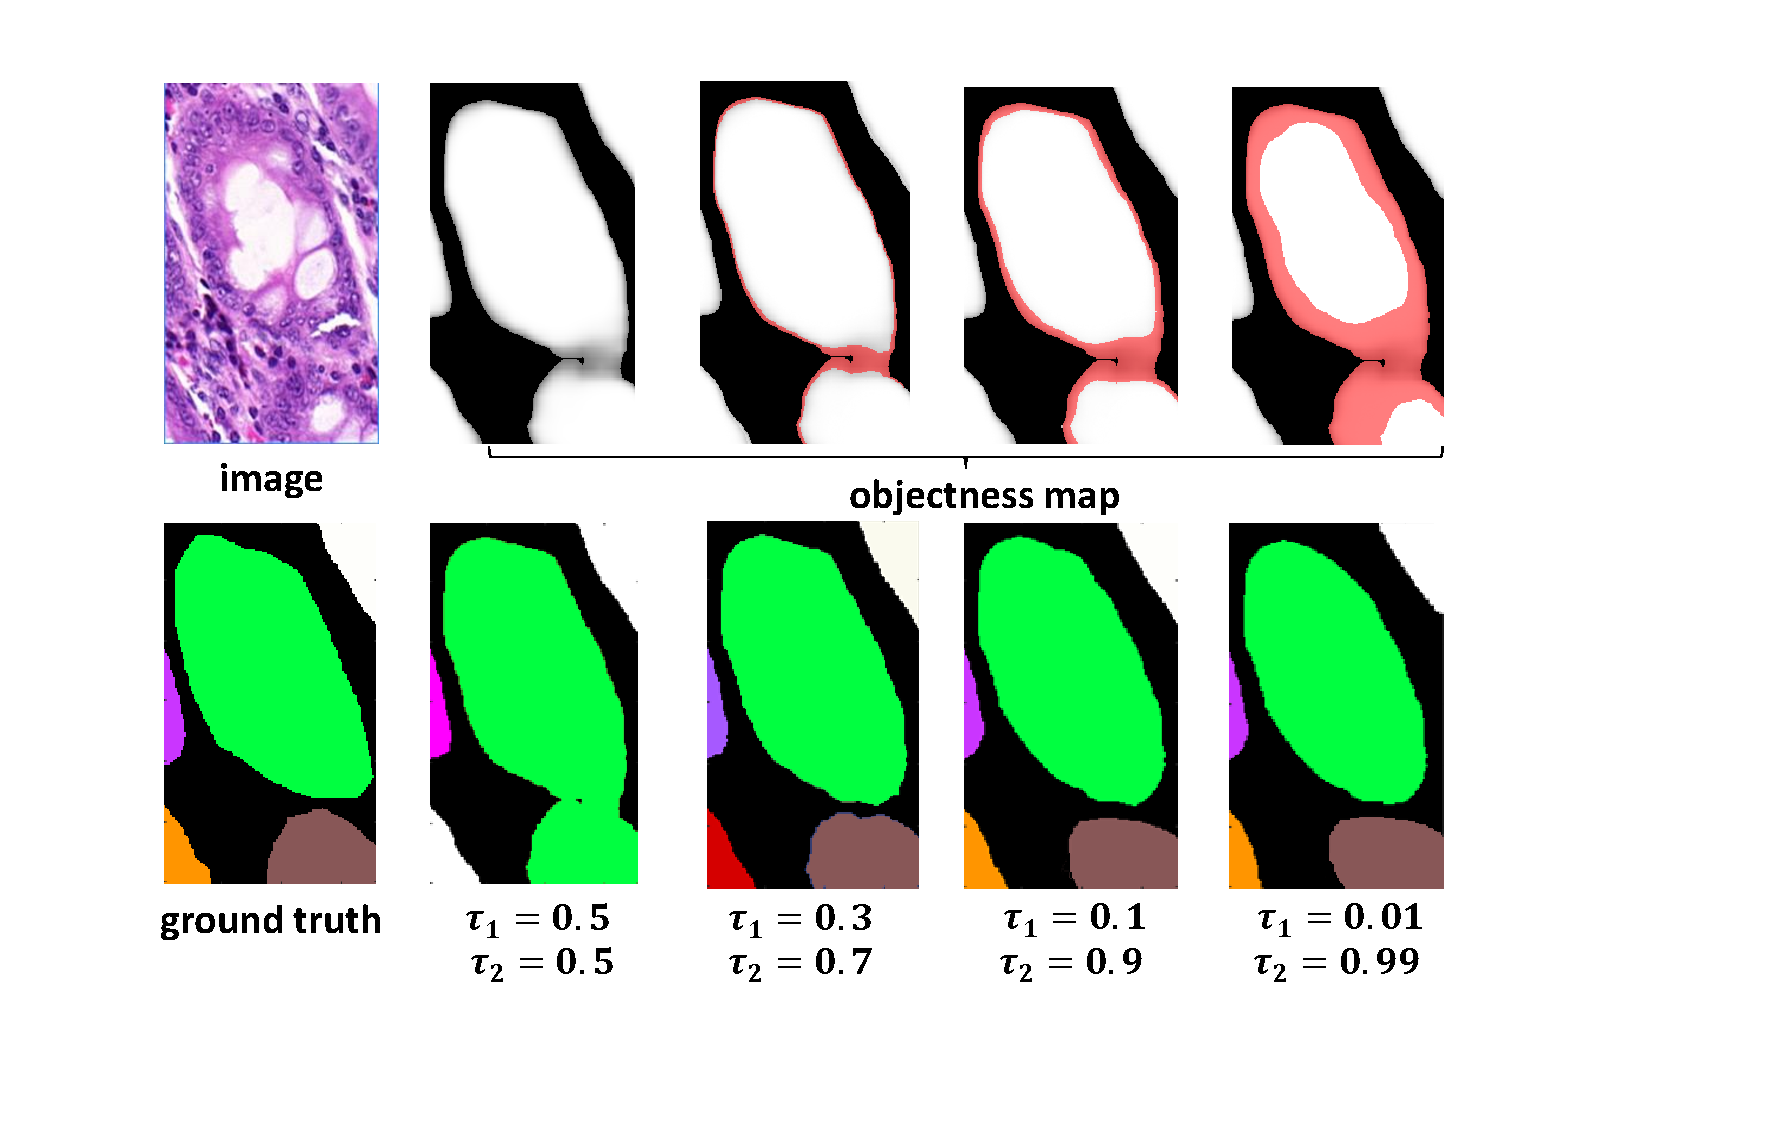
\includegraphics[width=3.4in]{figures/FigFusion.pdf}
   %\includegraphics[width=0.8\linewidth]{egfigure.eps}
    \end{center}
    \caption{Diagram of effects of varying $[\tau_1,\tau_2]$ to final segmentation.
        With $[\tau_1,\tau_2]$ increasing, the ambiguous region (marked red in top objectness map) becomes larger, leading to a stronger ellipse constraint on object shape.}
    \label{FigFusion}
\end{figure}